\documentclass[]{article}
\usepackage[round]{natbib}

\usepackage{fullpage}
\usepackage{listings}
\usepackage{url}
\usepackage{authblk}
\usepackage{graphicx}
\usepackage{color}

% lorem ipsum dummy text
\usepackage{lipsum}

\lstset{language=Python}

% local definitions
\newcommand{\comment}[1]{{\textcolor{red}{Comment: #1}}}

% cross-reference with supplement
\usepackage{xr}
\externaldocument{supplement}

\begin{document}

\title{A weakly structured stem for human origins in Africa}
\author[1]{Aaron P. Ragsdale}
\author[2]{Timothy D. Weaver}
\author[3]{Elizabeth G. Atkinson}
\author[4]{Eileen Hoal}
\author[5]{Marlo M\"{o}ller}
\author[2,6,*]{Brenna M. Henn}
\author[7,**]{Simon Gravel}
\affil[1]{FIXME: UW Madison}
\affil[2]{Department of Anthropology, University of California, Davis, Davis, CA 95616, USA}
\affil[3]{FIXME: DSI-NRF Centre of Excellence for Biomedical Tuberculosis Research; South African Medical Research Council Centre for Tuberculosis Research; Division of Molecular Biology and Human Genetics, Faculty of Medicine and Health Sciences, Stellenbosch University, Cape Town, South Africa}
\affil[4]{FIXME}
\affil[5]{FIXME}
\affil[6]{UC Davis Genome Center, University of California, Davis, Davis, CA 95616, USA}
\affil[7]{FIXME: McGill}
\affil[*]{bmhenn@ucdavis.edu}
\affil[**]{simon.gravel@mcgill.ca}
\maketitle

\abstract{
A very simple template for an article class document.
}

\section*{Introduction}

\section*{Results}

\begin{figure}[ht]
\begin{center}
\makebox[\textwidth][c]{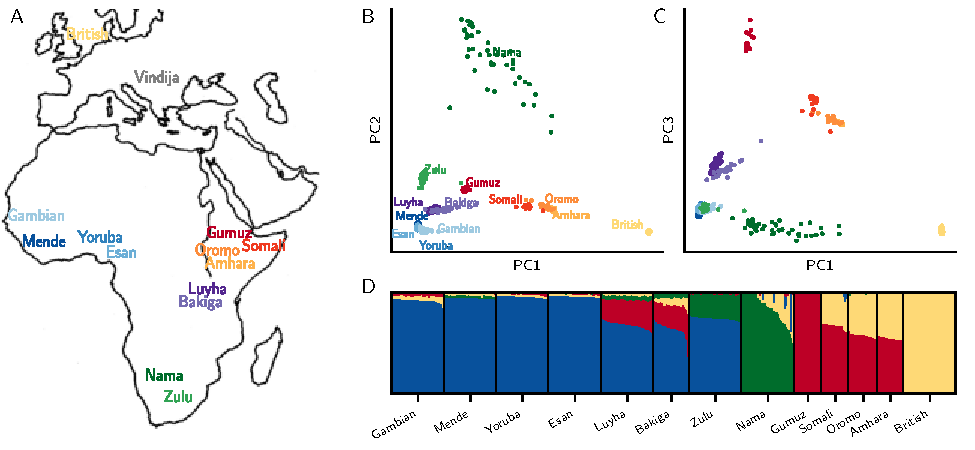
\includegraphics{figures/fig1.pdf}}
\caption{\textbf{The first figure}.
    It has a caption.
}
\label{fig:1}
\end{center}
\end{figure}

\subsection*{A Late Middle Stone Age common ancestry for contemporary human populations}

\subsection*{Evidence for deep population structure, but not archaic admixture within Africa}

\subsection*{Reconciling multiple lines of genetic evidence}

\section*{Discussion}

\subsection*{The Middle Stone Age in Africa}

\subsection*{Contrasting archaic admixture and a weakly structured stem}

\section*{Methods}
\cite{Kelleher2016-lw}

\section*{Acknowledgements}

\break

\bibliographystyle{plainnat}
\bibliography{paper}
\end{document}
